\section{Appendix}
\label{app:models}

\textbf{Model and action interfaces.} Table~\ref{tab:models} summarises the
three structured decision models discussed in the paper. Only Laya and Vela are
run locally; Jev defines the commercial reference point and is not evaluated
here.

\begin{table*}[t]
\centering
\small
\caption{The three structured decision models discussed in this paper. Only
Laya and Vela are run locally; Jev defines the commercial reference point and
is not evaluated here.}
\label{tab:models}
\begin{tabular}{@{}p{1.5cm}p{4.1cm}p{4.6cm}p{4.4cm}@{}}
\toprule
Model & Interface & Training route & Role in this study \\
\midrule
Jev & One call returns typed \textsc{Noul}, \textsc{Choice} and \textsc{Score} decisions with probabilities & TypeSafe names RLCD and a proper-scoring objective; the full recipe is not public & Reference point for the RLCD / System One family; not run \\
Laya 0.4.16 & ModernBERT-large encoder with decision heads, $\approx$421M parameters; \textsc{Noul}, \textsc{Choice}, \textsc{Score} & Upstream describes the recipe as RLCD with log, spherical and ranked probability scores & Open RLCD model used in all experiments \\
Vela 2.0 0.3B & 22-layer ModernBERT, 768 hidden, 8{,}192 tokens; \textsc{Noul}, \textsc{Choice}, \textsc{Score}, \textsc{Span}, \textsc{Set} & Initialised from Decision-1.0-Kai Choice path, task-specific losses, routing data; not called RLCD & Interface-matched comparison model with a different recipe \\
\bottomrule
\end{tabular}
\end{table*}


\label{app:native}

\textbf{Native single-action baselines.} Table~\ref{tab:native} reports the
accuracy and mean per-call latency of the two native actions on the
\texttt{search\_dev} pools. These numbers define the fixed policies that every
searched policy is compared against. The two representations have similar
per-call cost, which is why the fitness function uses call count rather than a
model-specific latency term. Peak resident memory is included to document the
CPU-only execution envelope.

\begin{table*}[t]
\centering
\small
\caption{Native single-action baselines on the 60-row selection pools
(\texttt{search\_dev}, seed 17). Latency is the per-call mean on the local CPU
and is reported only to show that the two representations cost roughly the
same; it is not used in the fitness function.}
\label{tab:native}
\begin{tabular}{@{}llrrrrrr@{}}
\toprule
Task & Model & $n$ & \textsc{Noul} acc. & \textsc{Choice} acc. & \textsc{Noul} ms & \textsc{Choice} ms & Peak RSS (MB) \\
\midrule
CodeXGLUE & Laya & 60 & 0.450 & 0.650 & 2304 & 2239 & 2114 \\
CodeXGLUE & Vela & 60 & 0.633 & 0.667 & 2437 & 2341 & 1931 \\
FinDVer & Laya & 59 & 0.712 & 0.644 & 2768 & 2741 & 2117 \\
FinDVer & Vela & 59 & 0.458 & 0.458 & 2394 & 2263 & 1795 \\
ProcessBench & Laya & 60 & 0.100 & -- & 2616 & -- & 2124 \\
ProcessBench & Vela & 60 & 0.100 & -- & 1577 & -- & 1747 \\
\bottomrule
\end{tabular}
\end{table*}


\label{app:extra}

\textbf{Complementarity overview.} Figure~\ref{fig:headroom} visualises the
gross and net repair counts behind Table~\ref{tab:complementarity}, including
the train-selected direction applied unchanged to dev and confirm.

\begin{center}
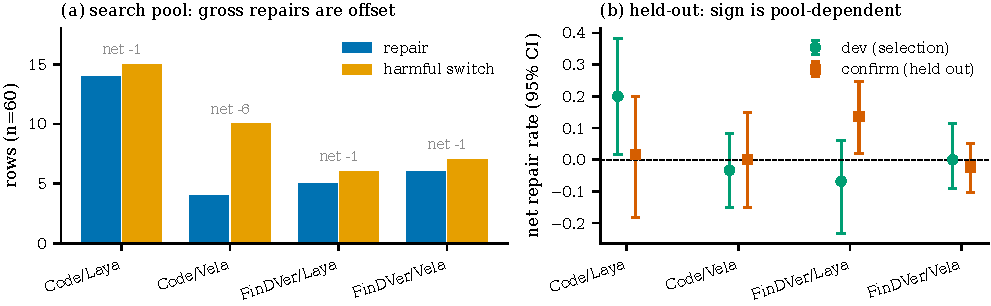
\includegraphics[width=0.86\linewidth]{figures/fig_headroom.pdf}
\captionof{figure}{Action complementarity. (a) On the training pool, the second
action repairs errors but also breaks correct answers; the net count is printed
above each pair. (b) The same train-selected direction applied to dev and
confirm: the sign of net repair changes across pools, and only one confirm cell
has an interval above zero.}
\label{fig:headroom}
\end{center}

\textbf{Repair profile.} Figure~\ref{fig:repair} shows the repair rate of the
second action as a function of the \noul{} probability bin, separately for the
training, dev and confirm pools. Each point is the fraction of rows in that bin
where \noul{} was wrong and \choice{} was correct. Bin counts are printed when
at least eight rows fall in the bin. The figure motivates the claim in
Section~\ref{sec:results} that repairs concentrate at mid and high probability
rather than in the low-confidence tail.

\begin{center}
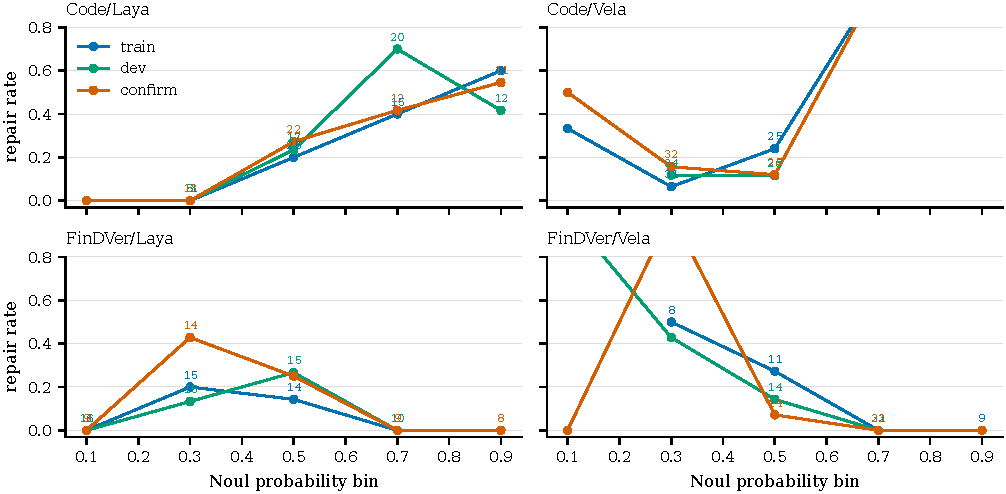
\includegraphics[width=0.92\linewidth]{figures/fig_repair_profile.pdf}
\captionof{figure}{Repair rate by \noul{} probability bin for the four binary
cells. Repairs are rare in the lowest bin and concentrate around
$p\in[0.4,0.8]$, where a confidence cascade is least likely to switch.}
\label{fig:repair}
\end{center}

\textbf{Calibration details.} Table~\ref{tab:calibration} reports calibration
and its relation to routing; Figure~\ref{fig:calibration} plots reliability
diagrams on confirm for the four binary cells, before and after temperature
scaling. The scaling parameters are fitted on \texttt{search\_train} and applied
unchanged to confirm. Because temperature scaling is monotone, it changes the
numerical probabilities but not the ordering of rows, and therefore not the set
of band policies available to the router.

\begin{table*}[t]
\centering
\small
\caption{Calibration on \texttt{confirm} and its relation to routing.
Temperature $T$ is fitted on \texttt{search\_train}; ECE uses 15 equal-width
bins. Gold AUROC is the probability's ability to rank current-action
correctness; repair AUROC is its ability to rank rows that the second action
would fix. The last two columns are the net repair of a band policy selected
on \texttt{search\_dev} with raw and temperature-scaled probabilities.}
\label{tab:calibration}
\begin{tabular}{@{}lrrrrrrrr@{}}
\toprule
Task / model & ECE raw & ECE $T$ & Brier raw & Brier $T$ & AUROC gold & AUROC repair & Route raw & Route $T$ \\
\midrule
CodeXGLUE / Laya & 0.230 & 0.076 & 0.287 & 0.250 & 0.550 & 0.791 & -5.0 & -1.7 \\
CodeXGLUE / Vela & 0.090 & 0.045 & 0.260 & 0.250 & 0.522 & 0.444 & +0.0 & +1.7 \\
FinDVer / Laya & 0.290 & 0.141 & 0.285 & 0.246 & 0.603 & 0.336 & +2.3 & +0.0 \\
FinDVer / Vela & 0.147 & 0.169 & 0.218 & 0.234 & 0.605 & 0.095 & -2.3 & +0.0 \\
\bottomrule
\end{tabular}
\end{table*}


\begin{center}
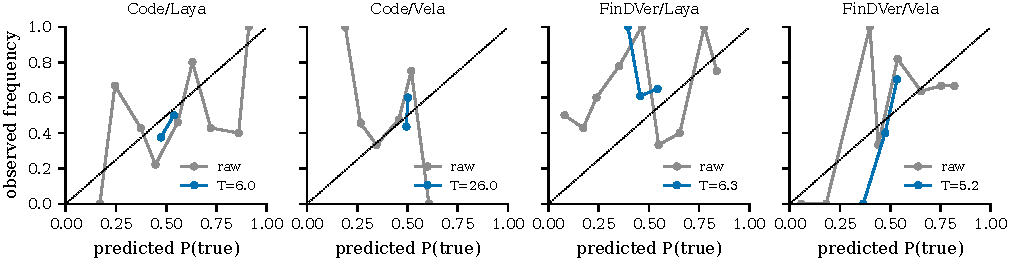
\includegraphics[width=0.92\linewidth]{figures/fig_calibration.pdf}
\captionof{figure}{Reliability diagrams on the confirm pool for the four binary
cells. Grey is the raw \noul{} probability, blue is temperature-scaled.
Temperature scaling reduces the calibration error, but it is a monotone map:
the ordering of rows, and therefore the set of band policies available up to a
reparameterisation, is unchanged.}
\label{fig:calibration}
\end{center}

\textbf{Search diagnostics.} Figure~\ref{fig:search} collects the three
trajectory diagnostics discussed in Section~\ref{sec:results}: the neutral
mutation rate, the rank correlation between training and dev fitness across the
archive, and best-so-far training fitness for seed 17.

\begin{center}
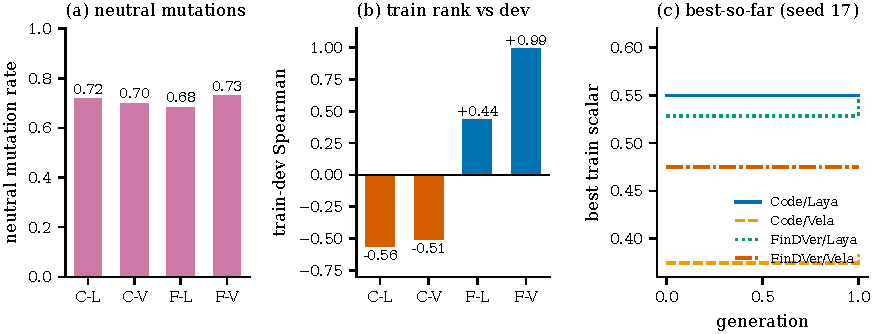
\includegraphics[width=0.92\linewidth]{figures/fig_search.pdf}
\captionof{figure}{Search diagnostics. (a) Between 68\% and 73\% of single-gene
mutations leave training fitness unchanged. (b) Rank correlation between
training and dev fitness across the archive is negative for both CodeXGLUE cells
and positive for FinDVer. (c) Best-so-far training fitness for seed 17; most
runs improve at most once, and several are flat from generation zero.}
\label{fig:search}
\end{center}

\textbf{Ranking versus policy value.} Figure~\ref{fig:predictability} plots
out-of-fold AUROC against the confirm net utility of the frozen dev-selected
policy for each cell. Points to the right of 0.5 have ranking signal; points
below zero have negative policy value. The dissociation is visible: the cell
with the strongest ranking signal (FinDVer/Vela) has a negative confirm net, and
the cell with the best confirm net (FinDVer/Laya) has near-chance ranking
signal.

\label{app:boundary}

\textbf{Boundary checks.} Table~\ref{tab:boundary} reports the transfer counts
and the four highest-severity fault-map cells. Figure~\ref{fig:faultmap} shows
the full confirm-pool severity map by task, model and confidence band.

\begin{table*}[t]
\centering
\small
\caption{Boundary checks. Top: frozen-genome transfer, counting significant
paired accuracy differences against the target's fixed switch-only policy;
diagonal cells are same-task deployment checks, off-diagonal cells are true
transfer. Bottom: the four highest-severity fault-map cells, with severity
defined as the error rate in the cell.}
\label{tab:boundary}
\begin{tabular}{@{}lrr@{}}
\toprule
Transfer & Sig. positive & Sig. negative \\
\midrule
Diagonal (same task) & 0 & 2 \\
Off-diagonal (true transfer) & 0 & 4 \\
\bottomrule
\end{tabular}

\vspace{4pt}
\begin{tabular}{@{}lrrrrrr@{}}
\toprule
Fault-map cell & $n$ disc. & Severity & $n$ dev & Severity & $n$ conf. & Severity \\
\midrule
ProcessBench / Vela / mid & 14 & 0.929 & 10 & 0.800 & 12 & 0.833 \\
ProcessBench / Laya / mid & 13 & 0.923 & 15 & 0.867 & 16 & 0.875 \\
ProcessBench / Vela / low & 45 & 0.889 & 46 & 0.957 & 47 & 0.936 \\
ProcessBench / Laya / high & 41 & 0.756 & 35 & 0.914 & 38 & 0.895 \\
\bottomrule
\end{tabular}
\end{table*}


\begin{center}
\begin{minipage}[t]{0.48\linewidth}
\centering
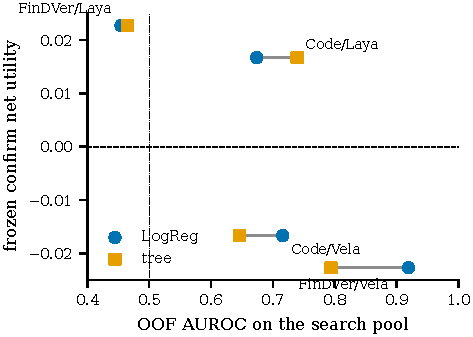
\includegraphics[width=\linewidth]{figures/fig_predictability.pdf}
\captionof{figure}{OOF AUROC versus confirm net utility. The dashed horizontal
line is zero net utility; the dotted vertical line is chance-level AUROC.
Ranking quality and policy value are not the same quantity.}
\label{fig:predictability}
\end{minipage}\hfill
\begin{minipage}[t]{0.48\linewidth}
\centering
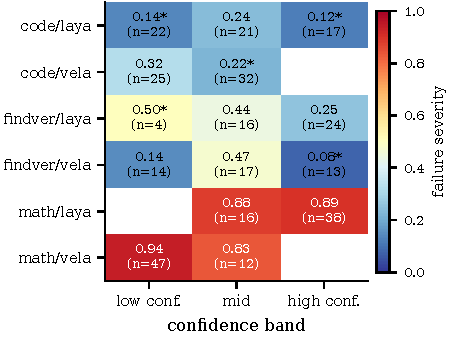
\includegraphics[width=\linewidth]{figures/fig_faultmap.pdf}
\captionof{figure}{Confirm-pool failure severity by task, model and confidence
band. Asterisks mark cells that were not confirmed within the 0.15 tolerance.
The stable high-severity region is the mid-confidence band on ProcessBench,
where both representations fail together.}
\label{fig:faultmap}
\end{minipage}
\end{center}

\textbf{Reproducibility details.} All results in this paper are derived from
committed JSON files. The per-row caches are one JSON file per pool, named
\texttt{cache\_<split>\_<task>\_<model>.json} under
\texttt{results/v4/evolution/}; the analyses are produced by
\texttt{scripts/analyze\_action\_\allowbreak complementarity.py},
\texttt{analyze\_complementarity\_heldout.py},
\texttt{analyze\_utility\_predictability.py},
\texttt{analyze\_search\_landscape.py},
\texttt{analyze\_transfer\_heldout.py},
\texttt{analyze\_calibration.py},
\texttt{analyze\_seed\_extension.py},
\texttt{analyze\_fixed\_action\_cis.py} and
\texttt{analyze\_search\_dynamics.py}. The tables are generated by
\texttt{scripts/make\_paper\_tables.py} and the figures by
\texttt{scripts/plot\_paper\_figures.py}; neither script contains a hand-copied
number. The GA/ES/NSGA-II runners are in \texttt{src/evolution/}. Model
revisions, dataset revisions, seeds and CPU thread counts are recorded in each
result file's metadata. The five-seed extension uses seeds 17, 23, 41, 59 and
73; the budget probe uses the same cache with a cap of 48 unique genomes. No
hosted CI runner is used: every model call was executed on the local Windows
machine, and the cached outputs are the only inputs to the analyses reported
here.

\textbf{What is not reported.} The locked test was not run, the \noul{} template
was not audited against alternative wordings, real end-to-end latency was not
measured for every searched policy, and Jev was not evaluated. These omissions
are stated in the main text and are not filled with proxy numbers. The
FinDVer/Laya confirm cell is the only cell with a positive net-repair accuracy
interval; it should be treated as a lead for a larger replication, not as a
deployable result.
